\subsection{导数应用}

	\begin{ti}
		曲线 $\begin{cases}
			x = \ee^{t} \sin 2t,\\
			y = \ee^{t} \cos t
		\end{cases}$ 在点 $t = 0$ 处的切线方程为\htwo.
	\end{ti}

	\begin{ti}
		若曲线 $C: y = f(x)$ 由方程
		\[
			2x - y = 2\arctan(y - x)
		\]
		确定,则曲线 $C$ 在点 $\left( 1 + \frac{\uppi}{2}, 2 + \frac{\uppi}{2} \right)$ 处的切线方程是 $y = $\htwo.
	\end{ti}

	\begin{ti}
		曲线 $r = \cos 2 \theta$ 在 $\theta = \frac{\uppi}{4}$ 处的切线方程为\htwo.
	\end{ti}

	\begin{ti}
		已知曲线的极坐标方程 $r = 1 - \cos \theta$,求曲线上对应于 $\theta = \frac{\uppi}{6}$ 处的切线与法线的直角坐标方程.
	\end{ti}

	\begin{ti}
		已知两曲线由 $y = f(x)$ 与 $xy + \ee^{x + y} = 1$ 所确定,且在点 $(0,0)$ 处的切线相同,写出此切线方程,并求极限 $\lim_{n \to \infty} n f\left( \frac{2}{n} \right)$.
	\end{ti}

	\begin{ti}
		设 $y = f(x)$ 由参数方程 $\begin{cases}
			x = 1 + t^{2},\\
			y = \cos t
		\end{cases}$ 所确定,求曲线 $y = y(x)$ 在 $t = \frac{\uppi}{2}$ 对应点处的切线方程.
	\end{ti}

	\begin{ti}
		设周期函数 $f(x)$ 在 $(-\infty,+\infty)$ 内可导,周期为 $4$,又 $\lim_{x \to 0} \frac{f(1) - f(1 - x)}{2x} = -1$,则曲线 $y = f(x)$ 在点 $(5,f(5))$ 处的切线斜率为\kuo.
		
		\fourch{$\frac{1}{2}$}{$0$}{$-1$}{$-2$}
	\end{ti}

	\begin{ti}
		设曲线 $f(x) = x^{n}$ 在点 $(1,1)$ 处的切线与 $x$ 轴的交点为 $(x_{n},0),n = 1,2,\cdots$,求 $\lim_{n \to \infty} f(x_{n})$.
	\end{ti}

	\begin{ti}
		曲线 $\left( 2 - x^{n^{2}} \right) y = 1$ 在点 $(1,1)$ 处的切线与 $x$ 轴的交点为 $(x_{n},0),n = 1,2,\cdots$,则 $\lim_{n \to \infty} x_{n}^{\frac{n^{2}}{2}} = $\htwo.
	\end{ti}

	\begin{ti}
		设 $y = \tan^{n}x$ 在 $x = \frac{\uppi}{4}$ 处的切线在 $x$ 轴上的截距为 $x_{n}$,试求 $\lim_{n \to \infty} y(x_{n})$.
	\end{ti}

	\begin{ti}
		已知 $f(x)$ 是周期为 $5$ 的连续函数,它在 $x = 0$ 的某邻域内满足关系式
		\[
			f(1 + \sin x) - 3 f(1 - \sin x) = 8x + \alpha(x),
		\]
		其中 $\alpha(x)$ 是当 $x \to 0$ 时比 $x$ 高阶的无穷小,且 $f(x)$ 在 $x = 1$ 处可导,求 $y = f(x)$ 在点 $(6,f(6))$ 处的切线方程.
	\end{ti}

	\begin{ti}
		在左半平面 $(x < 0)$ 上,求曲线 $y = \frac{1}{x}$ 和 $y = x^{2}$ 的公切线.
	\end{ti}

	\begin{ti}
		求双曲线 $y_{1} = \frac{1}{x}$ 与抛物线 $y_{2} = \sqrt{x}$ 的交角.
	\end{ti}

	\begin{ti}
		设函数 $f(x)$ 在 $x = 2$ 处可微,且满足
		\[
			2f(2 + x) + f(2 - x) = 3 + 2x + o(x),
		\]
		这里 $o(x)$ 表示比 $x$ 高阶的无穷小(当 $x \to 0$ 时),试求微分 $\left. \dd{f(x)} \right|_{x = 2}$,并求曲线 $y = f(x)$ 在点 $(2,f(2))$ 处的切线方程.
	\end{ti}

	\begin{ti}
		若函数 $f(x) = a \sin x + \frac{1}{3} \sin 3x$ 在 $x = \frac{\uppi}{3}$ 处取得极值,则 $a = $\htwo.
	\end{ti}

	\begin{ti}
		若 $f(x)$ 在 $x_{0}$ 点至少二阶可导,且
		\[
			\lim_{x \to x_{0}} \frac{f(x) - f(x_{0})}{(x - x_{0})^{2}} = -1,
		\]
		则函数 $f(x)$ 在 $x = x_{0}$ 处\kuo.
		
		\twoch{取得极大值}{取得极小值}{无极值}{不一定有极值}
	\end{ti}

	\begin{ti}
		设 $f(x)$ 在 $x = 0$ 的某邻域内连续且在 $x = 0$ 处存在二阶导数 $f''(0)$. 又设
		\[
			\lim_{x \to 0} \frac{\int_{0}^{x} t f(x - t) \dd{t}}{x^{4}} = a(\text{常数}\  a > 0),
		\]
		则\kuo.
		
		\onech{$x = 0$ 不是 $f(x)$ 的驻点}{$x = 0$ 是 $f(x)$ 的驻点,但不是 $f(x)$ 的极值点}{$x = 0$ 是 $f(x)$ 的极小值点}{$x = 0$ 是 $f(x)$ 的极大值点}
	\end{ti}

	\begin{ti}
		设函数 $y = y(x)$ 是由方程 $\begin{cases}
			x = 2t + |t|,\\
			y = 5t^{2} + 4t|t|
		\end{cases}$ 所确定. 在 $t = 0$ 处,函数 $y = y(x)$ \kuo.
		
		\onech{导数存在,但 $y'(0) \ne 0$}{导数 $y'(0) = 0$,但不是极值点}{是极小值点}{是极大值点}
	\end{ti}

	\begin{ti}
		已知 $f'(-x) = x\left[ f'(x) + 1 \right]$,求 $f(x)$ 的极值点,并说明是极大值点还是极小值点.
	\end{ti}

	\begin{ti}
		设函数 $f(x)$ 可导,且满足 $xf'(x) = f'(-x) + 1$,$f(0) = 0$,求:
		\begin{enumerate}
			\item $f'(x)$;
			\item 函数 $f(x)$ 的极值.
		\end{enumerate}
	\end{ti}

	\begin{ti}
		求函数 $f(x) = |x| \ee^{-|x - 1|}$ 的极值.
	\end{ti}

	\begin{ti}
		求函数 $f(x) = \begin{cases}
			x^{2x}, & x > 0,\\
			x + 2, & x \leq 0
		\end{cases}$ 的单调区间和极值.
	\end{ti}

	\begin{ti}
		设 $f(x) = f(-x)$,且在 $(0,+\infty)$ 内二阶可导,又 $f'(x) > 0$,$f''(x) < 0$,则 $f(x)$ 在 $(-\infty,0)$ 内的单调性和图形的凹凸性是\kuo.
		
		\twoch{单调增加,凸}{单调减少,凸}{单调增加,凹}{单调减少,凹}
	\end{ti}

	\begin{ti}
		设函数 $y = y(x)$ 由参数方程
		\[
			\begin{cases}
				x = t^{3} + 9t,\\
				y = t^{2} - 2t
			\end{cases}
		\]
		确定,求曲线 $y = y(x)$ 的凹区间.
	\end{ti}

	\begin{ti}
		设函数 $f(x)$ 在 $(-\infty,+\infty)$ 内连续,其一阶导函数 $f'(x)$ 的图形如图~\ref{fig:1.2.1} 所示,并设在 $f'(x)$ 存在处 $f''(x)$ 亦存在,则函数 $f(x)$ 及曲线 $y = f(x)$\kuo.
		
		\onech{只有 $1$ 个极大值点与 $1$ 个拐点}{有 $1$ 个极小值点,$1$ 个极大值点与 $1$ 个拐点}{有 $1$ 个极小值点,$1$ 个极大值点与 $2$ 个拐点}{有 $1$ 个极小值点,$1$ 个极大值点与 $3$ 个拐点}
		\begin{figure}[htbp]
			\centering
			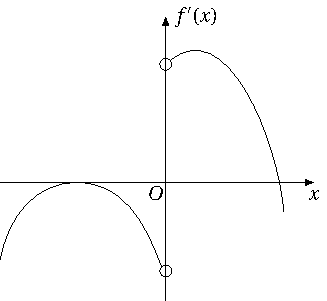
\includegraphics[scale=1]{figure/fig1-2-1.pdf}
			\caption{}\label{fig:1.2.1}
		\end{figure}
	\end{ti}

	\begin{ti}
		当 $x > 0$ 时,曲线 $y = x \sin\frac{1}{x}$ \kuo.
		
		\onech{有且仅有水平渐近线}{有且仅有铅直渐近线}{既有水平渐近线,也有铅直渐近线}{既无水平渐近线,也无铅直渐近线}
	\end{ti}

	\begin{ti}
		曲线 $y = \ln\left( \ee - \frac{1}{x} \right)$ 的全部渐近线为\htwo.
	\end{ti}

	\begin{ti}
		曲线 $y = \ee^{\frac{1}{x^{2}}} \arctan \frac{x^{2} + x + 1}{(x - 1)(x + 2)}$ 的渐近线有\kuo.
		
		\fourch{$1$ 条}{$2$ 条}{$3$ 条}{$4$ 条}
	\end{ti}

	\begin{ti}
		求 $y = \sqrt{4x^{2} + x} \ln\left( 2 + \frac{1}{x} \right)$ 的全部渐近线.
	\end{ti}

	\begin{ti}
		函数 $y = (x - 1)^{2} (x - 2)^{2} (-3 \leq x \leq 4)$ 的值域是
		
		\noindent\htwo.
	\end{ti}

	\begin{ti}
		设正值函数 $f(x)$ 在 $(1,+\infty)$ 内连续,求函数
		\[
			F(x) = \int_{1}^{x} \left[ \left( \frac{2}{x} + \ln x \right) - \left( \frac{2}{t} + \ln t \right) \right] f(t) \dd{t}
		\]
		的最小值点.
	\end{ti}

	\begin{ti}
		函数 $y = x^{x}$ 在区间 $\left[ \frac{1}{\ee},+\infty \right)$ 上\kuo.
		
		\onech{不存在最大值和最小值}{最大值是 $\ee^{\frac{1}{\ee}}$}{最大值是 $\left( \frac{1}{\ee} \right)^{\frac{1}{\ee}}$}{最小值是 $\left( \frac{1}{\ee} \right)^{\frac{1}{\ee}}$}
	\end{ti}

	\begin{ti}
		求函数 $f_{n}(x) = x^{n} \ee^{- n^{2} x}(n = 2,3,\cdots)$ 在 $[0,+\infty)$ 内的最值,并求极限 $\lim_{n \to \infty} f_{n}(x), x \geq 0$.
	\end{ti}

	\begin{ti}
		设 $f(x) = \begin{cases}
			\lim_{n \to \infty} \frac{1}{n} \sum_{k=0}^{n-1} \cos \frac{k}{n}x, & x > 0,\\
			1, & x = 0,\\
			f(-x), & x < 0.
		\end{cases}$
		\begin{enumerate}
			\item 求 $f'(0)$;
			\item 求 $f(x)$ 在 $[-\uppi,\uppi]$ 上的最大值.
		\end{enumerate}
	\end{ti}

	\begin{ti}
		设某物体的温度 $T$ 与时间 $t$ 满足函数关系:
		\[
			T = a\left( 1 - \ee^{-kt} \right) + b,
		\]
		其中 $T$ 的单位是 \si{\degreeCelsius},$t$ 的单位是 \si{min}. 现将该物体放入 \SI{200}{\degreeCelsius} 的高温介质中.
		\begin{enumerate}
			\item 若物体的初始温度是 \SI{20}{\degreeCelsius},求 $a$ 和 $b$;
			\item 若物体温度以 \SI{2}{\degreeCelsius/min} 的速率开始上升,求 $k$.
		\end{enumerate}
	\end{ti}

	\begin{ti}
		曲线 $y = y(x)$ 可表示为 $x = t^{3} - t, y = t^{4} + t$,$t$ 为参数. 证明:
		\begin{enumerate}
			\item $y = y(x)$ 在 $t = 0$ 处为拐点;
			\item $g(x) = \sqrt{\left( \frac{\dd{x}}{\dd{t}} \right)^{2} + \left( \frac{\dd{y}}{\dd{t}} \right)^{2}}$ 在 $t = 0$ 处取得极大值.
		\end{enumerate}
	\end{ti}

	\begin{ti}
		设有曲线弧 $y = \sin x(0 < x < \uppi)$.
		\begin{enumerate}
			\item 求出曲线弧的最小曲率半径;
			\item 求与曲线弧在曲率半径最小的点处相切且具有相同曲率和凹向的抛物线的方程.
		\end{enumerate}
	\end{ti}

	\begin{ti}
		曲线 $2y^{3} - 2y^{2} + 2xy - x^{2} = 1$ 在 $(1,1)$ 处的曲率半径为\htwo.
	\end{ti}

	\begin{ti}
		$y^{2} = 4x$ 在原点处的曲率圆方程为\htwo.
	\end{ti}

	\begin{ti}
		求曲线 $y = \ln x$ 上曲率最大的点,并在该点附近用抛物线 $y = ax^{2} + bx + c$ 近似代替 $y = \ln x$,求 $a,b,c$.
	\end{ti}

	\begin{ti}
		质点 $P$ 沿抛物线 $x = y^{2}(y > 0)$ 移动,$P$ 的横坐标 $x$ 的变化速度 \SI{5}{cm/s}. 当 $x = 9$ 时,点 $P$ 到原点 $O$ 的距离变化速度为\htwo.
	\end{ti}

	\begin{ti}
		半径为 $\frac{1}{2}$ 的圆在抛物线 $x = \sqrt{y}$ 凹的一侧上滚动.
		\begin{enumerate}
			\item 求圆心 $(\xi,\eta)$ 的轨迹方程.
			\item 当圆心以速率 $V_{0}$ 匀速上升时,求圆心的横坐标 $\xi$ 的增长速度.
		\end{enumerate}
	\end{ti}

	\begin{ti}
		球的半径以 \SI{5}{cm/s} 的速度匀速增长,问球的半径为 \SI{50}{cm} 时,球的表面积和体积的增长速度各是多少?
	\end{ti}